%Part of/Parte di https://github.com/f-dinucci/appuntiMeccanicaFluidi/
%License/Licenza Creative Commons Attribution-ShareAlike 4.0 International (CC BY-SA 4.0) - attribution/attribuzione Francesco Di Nucci
%See also/Vedere anche https://creativecommons.org/licenses/by-sa/4.0/ and/e https://creativecommons.org/licenses/by-sa/4.0/legalcode
%
\section{Proprietà dei fluidi}
%%SUBSECTION
\subsection{Densità}
Quanto visto prima per le proprietà conservate nei fluidi porta ad introdurre il concetto di densità: dividendo il volume di controllo in \textit{n} parti, ognuna con propri massa e volume, e prendendole via via più piccole, al limite conta solamente il rapporto massa/volume.
Per ogni grandezza conservata esiste una grandezza di densità, funzione continua delle variabili spaziali, ad esempio $\rho$ per la massa (alias si vede la massa come integrale della densità di massa):
	\begin{figure}[H]
		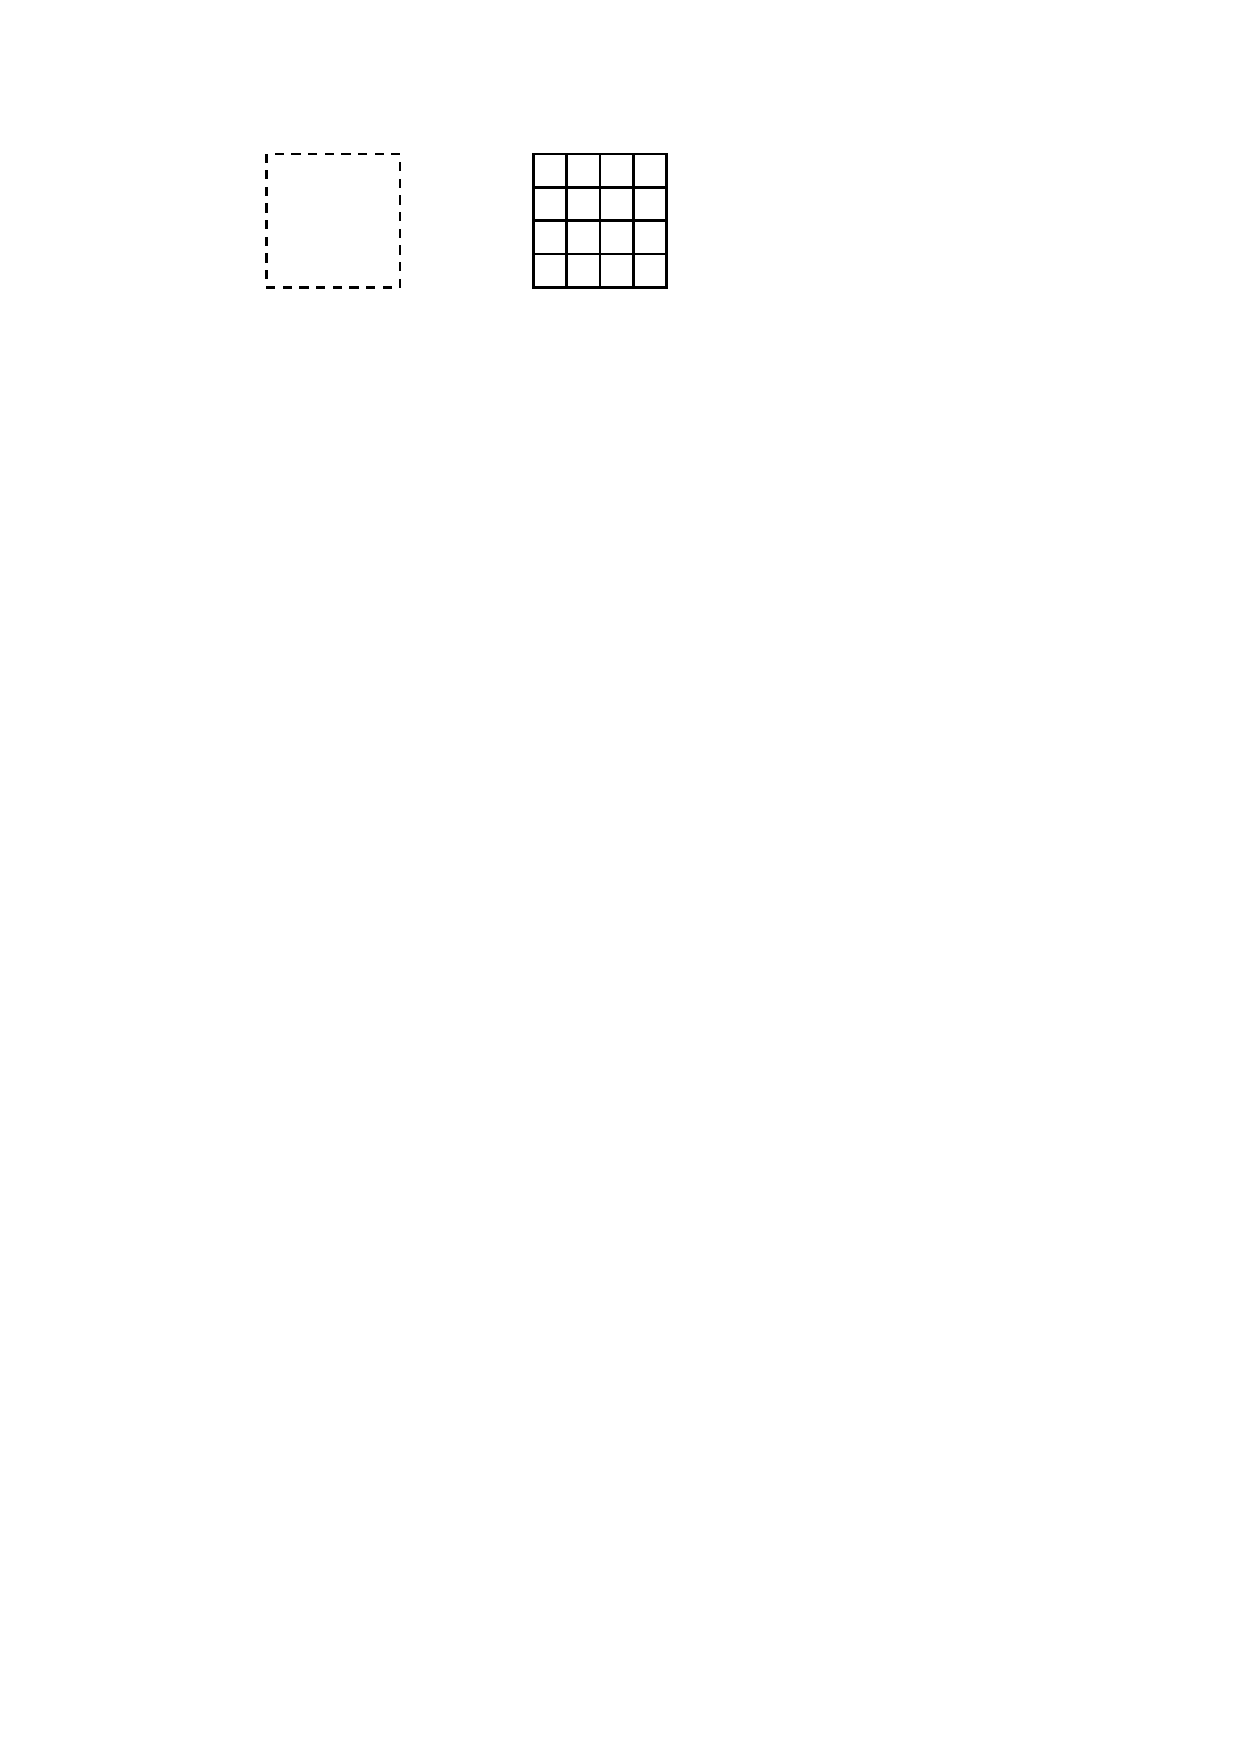
\includegraphics[scale=1.1]{./1.3 Proprietà dei fluidi/1.3-1}
		\centering
		\caption{Volume di controllo e suddivisione}
	\end{figure}
%
	\begin{equation*}
		M = \int_V {\rho \dd{V}}
	\end{equation*}
%
La densità di massa è tale che l'integrale dia la massa totale come risultato (è una sorta di definizione circolare):
%
	\begin{figure}[H]
		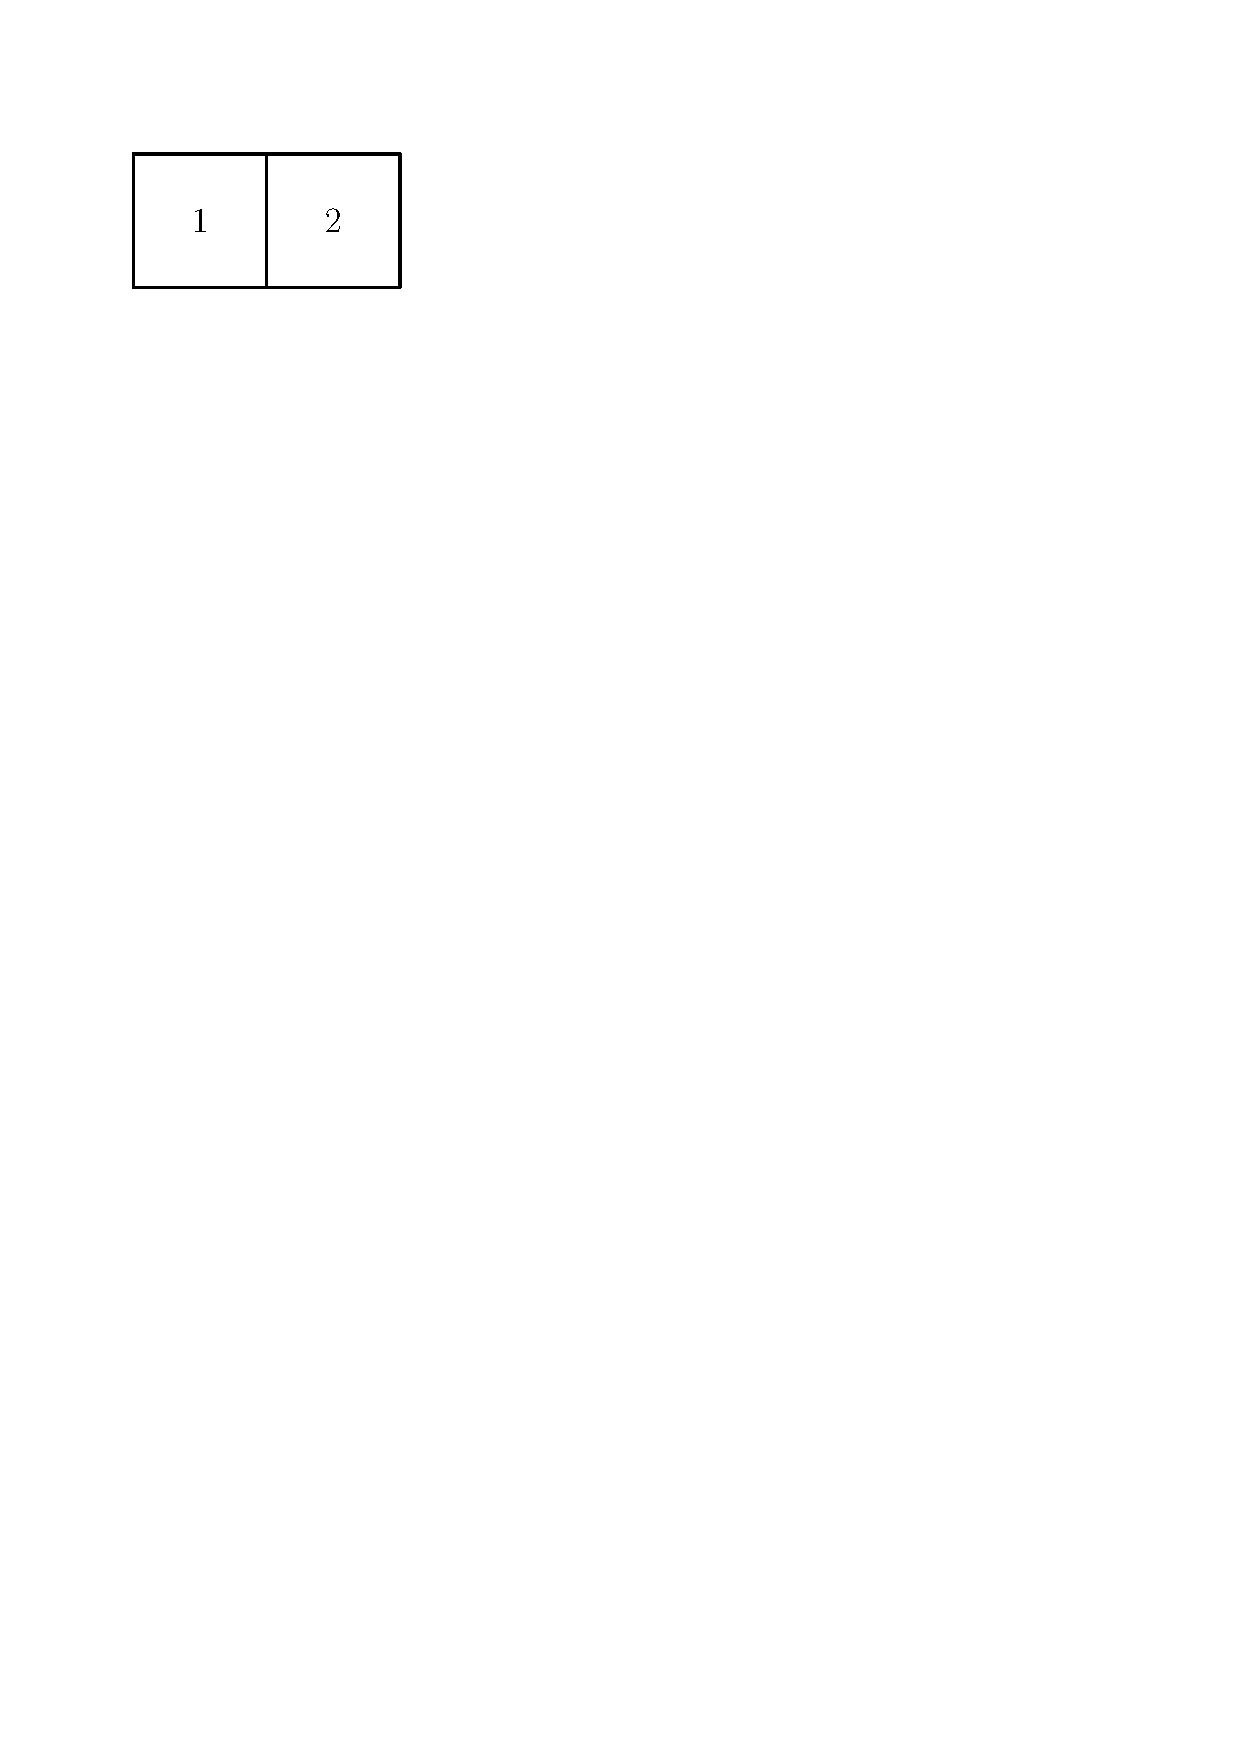
\includegraphics[scale=1]{./1.3 Proprietà dei fluidi/1.3-2}
		\centering
		\caption{Combinazione di due volumi di controllo}
	\end{figure}
%
Combinando due volumi di controllo si ha che la proprietà matematica dell'additività degli integrali coincide con la proprietà fisica della somme di due masse:
%
	\begin{equation*}
		\begin{gathered}
			\int_1 {\rho \dd{V}} + \int_2{\rho \dd{V}} = \int_{1+2}{\rho \dd{V}} \\
			\text{cioè} \\
			M_1 + M_2 = M_{1+2}
		\end{gathered}
	\end{equation*}
%
In piccolo la struttura della materia è discreta (molecole/atomi), non continua: il modello di corpo continuo si ferma a livello delle molecole ma è utile dato che data una generica densità \textit{f} permette di rappresentare ogni generica proprietà \textit{P} in un certo volume \textit{V} come:
%
	\begin{equation*}
		P_V = \int_V f(x, y, z, t) \dd{V}
	\end{equation*}
%
Il che è utile dato che una descrizione molecola per molecola sarebbe inutilizzabile a livello macroscopico. Da notare che i livelli microscopico e macroscopico non sono disgiunti, hanno un legame statistico/probabilistico: le proprietà macroscopiche possono essere definite come distribuzioni di probabilità di quelle microscopiche.
%
Prendendo il volume $V$, somma di due volumi $V_1$ e $V_2$, la proprietà P nel volume $V = V_1 + V_2$ è data dalla somma della proprietà $P$ in $V_1$ e $V_2$: si tratta quindi di grandezze estensive\footnote{dipendono cioè dalla dimensione/estensione del sistema, a differenza delle grandezze intensive (come la temperatura).}.
%
%%SUBSECTION
\subsection{Cammino libero medio}
In meccanica dei fluidi si utilizza il concetto di rapporti adimensionali: qualcosa è trascurabile se piccolo rispetto ad un termine di riferimento. Tenendo conto che nei fluidi le molecole scorrono, a differenza dei solidi nei quali sono ``incastrate'' in un reticolo, si definisce il \textit{cammino libero medio}.
In un fluido le molecole percorrono una certa distanza prima di collidere con un'altra e cambiare direzione, questa distanza è detta cammino libero medio, $\lambda$: se la lunghezza/diametro del volume di controllo è molto maggiore del cammino libero medio, cioè $L >> \lambda$, si è nell'ipotesi del continuo.
Di solito si considera valida l'ipotesi del continuo se il rapporto $\frac{\lambda}{L}$, detto \textit{numero di Knudsen}, è minore di 0.01.
Un caso ad esempio in cui questo va considerato è il volo spaziale: il cammino libero medio aumenta salendo nell'atmosfera, ad una certa altezza il veicolo non è più grande rispetto ad esso e bisogna abbandonare tutte le ipotesi relative alla meccanica del continuo.
Analogamente per i micromeccanismi, dove si ha che $L << \lambda$.
%
\subsection*{Bibliografia 1.3}
\cite[Cap.\ 2.1, 2.2]{CengelCimbala}\\
\cite[Cap.\ 1.3, pag.\ 8, 9, 15 ]{LuchiniQuadrio}\\
\cite[Cap.\ 1.2, 1.9]{PnueliGutfinger}